\documentclass[10pt]{article}
\usepackage{amsmath,amsthm,amssymb,graphicx,xspace,epsfig,xcolor,colortbl,diagbox}
\usepackage{tikz, tkz-graph, tkz-berge}
\usetikzlibrary{decorations.pathreplacing}
\usetikzlibrary{patterns}
\usetikzlibrary{patterns.meta}
\usetikzlibrary{automata,arrows,positioning,calc}
\usepackage{pgf}
\usepackage{pgffor}
\usepackage{color}
\usepackage{mathtools,amsfonts,amsthm,mathrsfs,amssymb,stmaryrd}
\usepackage{xcolor}

\begin{document}

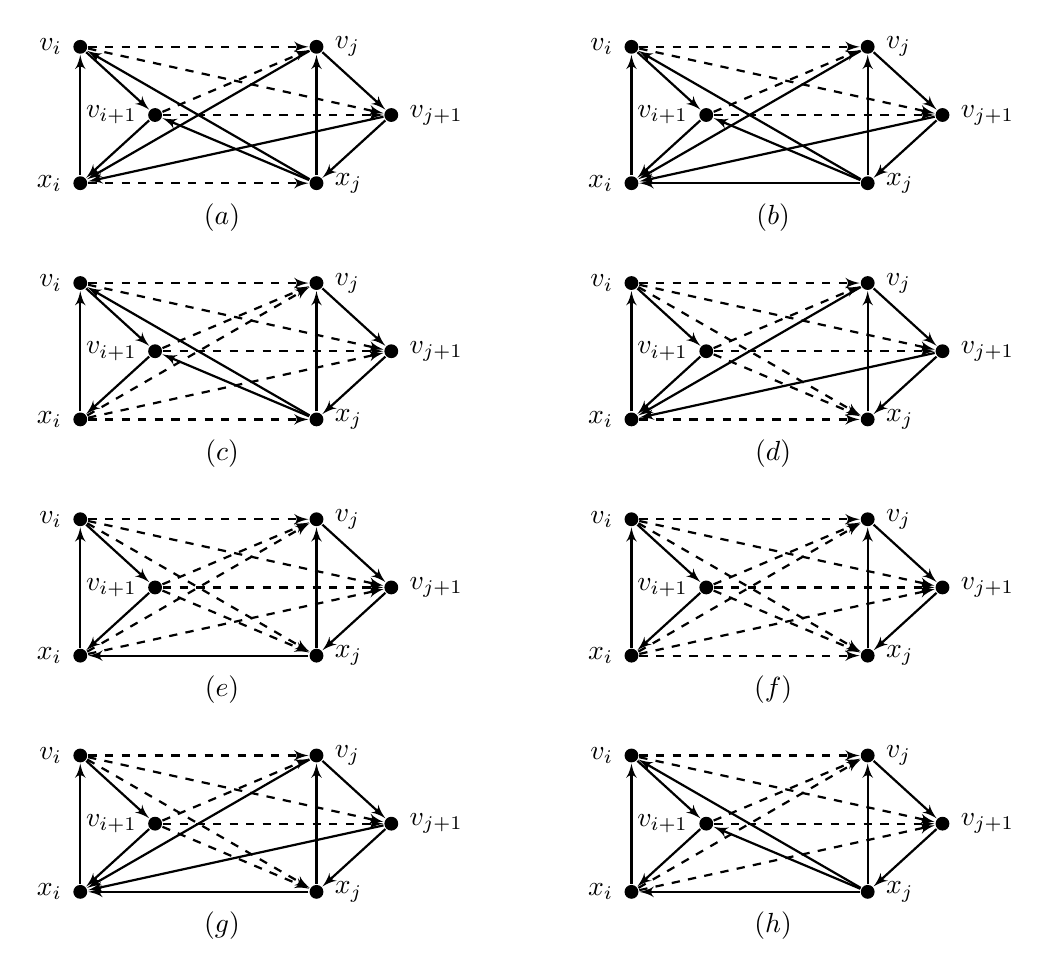
\begin{tikzpicture}[thick,scale=1, every node/.style={transform shape}]
  \tikzset{vertex/.style = {circle,fill=black,minimum size=5pt, inner sep=0pt}}
  \tikzset{edge/.style = {->,> = latex'}}
  \begin{scope}
      \node[vertex, label=left:$v_{i+1}$] (vip1) at (0:0.45) {};
      \node[vertex, label=left:$v_{i}$] (vi) at (120:1) {};
      \node[vertex, label=left:$x_{i}$] (xi) at (-120:1) {};
      \draw[edge] (xi) to (vi);
      \draw[edge] (vi) to (vip1);
      \draw[edge] (vip1) to (xi);

      \begin{scope}[xshift=3cm]
      \node[vertex, label=right:$v_{j+1}$] (vjp1) at (0:0.45) {};
      \node[vertex, label=right:$v_{j}$] (vj) at (120:1) {};
      \node[vertex, label=right:$x_{j}$] (xj) at (-120:1) {};
      \draw[edge] (xj) to (vj);
      \draw[edge] (vj) to (vjp1);
      \draw[edge] (vjp1) to (xj);
      \end{scope}

      \draw[edge,dashed] (xi) to (xj);
      \draw[edge,dashed] (vip1) to (vj);
      \draw[edge,dashed] (vip1) to (vjp1);
      \draw[edge,dashed] (vi) to (vj);
      \draw[edge,dashed] (vi) to (vjp1);

      \draw[edge] (vj) to (xi);
      \draw[edge] (vjp1) to (xi);
      \draw[edge] (xj) to (vi);
      \draw[edge] (xj) to (vip1);

      \node[] (a) at (1.3,-1.3) {$(a)$};
  \end{scope}
  \begin{scope}[xshift=7cm]
      \node[vertex, label=left:$v_{i+1}$] (vip1) at (0:0.45) {};
      \node[vertex, label=left:$v_{i}$] (vi) at (120:1) {};
      \node[vertex, label=left:$x_{i}$] (xi) at (-120:1) {};
      \draw[edge] (xi) to (vi);
      \draw[edge] (vi) to (vip1);
      \draw[edge] (vip1) to (xi);

      \begin{scope}[xshift=3cm]
      \node[vertex, label=right:$v_{j+1}$] (vjp1) at (0:0.45) {};
      \node[vertex, label=right:$v_{j}$] (vj) at (120:1) {};
      \node[vertex, label=right:$x_{j}$] (xj) at (-120:1) {};
      \draw[edge] (xj) to (vj);
      \draw[edge] (vj) to (vjp1);
      \draw[edge] (vjp1) to (xj);
      \end{scope}

      \draw[edge,dashed] (vip1) to (vj);
      \draw[edge,dashed] (vip1) to (vjp1);
      \draw[edge,dashed] (vi) to (vj);
      \draw[edge,dashed] (vi) to (vjp1);

      \draw[edge] (xj) to (xi);
      \draw[edge] (vj) to (xi);
      \draw[edge] (vjp1) to (xi);
      \draw[edge] (xj) to (vi);
      \draw[edge] (xj) to (vip1);

      \node[] (a) at (1.3,-1.3) {$(b)$};
  \end{scope}
  \begin{scope}[yshift=-3cm]
      \node[vertex, label=left:$v_{i+1}$] (vip1) at (0:0.45) {};
      \node[vertex, label=left:$v_{i}$] (vi) at (120:1) {};
      \node[vertex, label=left:$x_{i}$] (xi) at (-120:1) {};
      \draw[edge] (xi) to (vi);
      \draw[edge] (vi) to (vip1);
      \draw[edge] (vip1) to (xi);

      \begin{scope}[xshift=3cm]
      \node[vertex, label=right:$v_{j+1}$] (vjp1) at (0:0.45) {};
      \node[vertex, label=right:$v_{j}$] (vj) at (120:1) {};
      \node[vertex, label=right:$x_{j}$] (xj) at (-120:1) {};
      \draw[edge] (xj) to (vj);
      \draw[edge] (vj) to (vjp1);
      \draw[edge] (vjp1) to (xj);
      \end{scope}

      \draw[edge,dashed] (vip1) to (vj);
      \draw[edge,dashed] (vip1) to (vjp1);
      \draw[edge,dashed] (vi) to (vj);
      \draw[edge,dashed] (vi) to (vjp1);
      \draw[edge,dashed] (xi) to (vj);
      \draw[edge,dashed] (xi) to (xj);
      \draw[edge,dashed] (xi) to (vjp1);

      \draw[edge] (xj) to (vi);
      \draw[edge] (xj) to (vip1);

      \node[] (a) at (1.3,-1.3) {$(c)$};
  \end{scope}
  \begin{scope}[yshift=-3cm, xshift=7cm]
      \node[vertex, label=left:$v_{i+1}$] (vip1) at (0:0.45) {};
      \node[vertex, label=left:$v_{i}$] (vi) at (120:1) {};
      \node[vertex, label=left:$x_{i}$] (xi) at (-120:1) {};
      \draw[edge] (xi) to (vi);
      \draw[edge] (vi) to (vip1);
      \draw[edge] (vip1) to (xi);

      \begin{scope}[xshift=3cm]
      \node[vertex, label=right:$v_{j+1}$] (vjp1) at (0:0.45) {};
      \node[vertex, label=right:$v_{j}$] (vj) at (120:1) {};
      \node[vertex, label=right:$x_{j}$] (xj) at (-120:1) {};
      \draw[edge] (xj) to (vj);
      \draw[edge] (vj) to (vjp1);
      \draw[edge] (vjp1) to (xj);
      \end{scope}

      \draw[edge,dashed] (xi) to (xj);
      \draw[edge,dashed] (vip1) to (vj);
      \draw[edge,dashed] (vip1) to (vjp1);
      \draw[edge,dashed] (vi) to (vj);
      \draw[edge,dashed] (vi) to (vjp1);
      \draw[edge,dashed] (vi) to (xj);
      \draw[edge,dashed] (vip1) to (xj);

      \draw[edge] (vj) to (xi);
      \draw[edge] (vjp1) to (xi);

      \node[] (a) at (1.3,-1.3) {$(d)$};
  \end{scope}
  \begin{scope}[yshift=-6cm]
      \node[vertex, label=left:$v_{i+1}$] (vip1) at (0:0.45) {};
      \node[vertex, label=left:$v_{i}$] (vi) at (120:1) {};
      \node[vertex, label=left:$x_{i}$] (xi) at (-120:1) {};
      \draw[edge] (xi) to (vi);
      \draw[edge] (vi) to (vip1);
      \draw[edge] (vip1) to (xi);

      \begin{scope}[xshift=3cm]
      \node[vertex, label=right:$v_{j+1}$] (vjp1) at (0:0.45) {};
      \node[vertex, label=right:$v_{j}$] (vj) at (120:1) {};
      \node[vertex, label=right:$x_{j}$] (xj) at (-120:1) {};
      \draw[edge] (xj) to (vj);
      \draw[edge] (vj) to (vjp1);
      \draw[edge] (vjp1) to (xj);
      \end{scope}

      \draw[edge,dashed] (vip1) to (vj);
      \draw[edge,dashed] (vip1) to (vjp1);
      \draw[edge,dashed] (vi) to (vj);
      \draw[edge,dashed] (vi) to (vjp1);
      \draw[edge,dashed] (vi) to (xj);
      \draw[edge,dashed] (vip1) to (xj);
      \draw[edge,dashed] (xi) to (vj);
      \draw[edge,dashed] (xi) to (vjp1);

      \draw[edge] (xj) to (xi);

      \node[] (a) at (1.3,-1.3) {$(e)$};
  \end{scope}
  \begin{scope}[xshift=7cm,yshift=-6cm]
      \node[vertex, label=left:$v_{i+1}$] (vip1) at (0:0.45) {};
      \node[vertex, label=left:$v_{i}$] (vi) at (120:1) {};
      \node[vertex, label=left:$x_{i}$] (xi) at (-120:1) {};
      \draw[edge] (xi) to (vi);
      \draw[edge] (vi) to (vip1);
      \draw[edge] (vip1) to (xi);

      \begin{scope}[xshift=3cm]
      \node[vertex, label=right:$v_{j+1}$] (vjp1) at (0:0.45) {};
      \node[vertex, label=right:$v_{j}$] (vj) at (120:1) {};
      \node[vertex, label=right:$x_{j}$] (xj) at (-120:1) {};
      \draw[edge] (xj) to (vj);
      \draw[edge] (vj) to (vjp1);
      \draw[edge] (vjp1) to (xj);
      \end{scope}

      \draw[edge,dashed] (vip1) to (vj);
      \draw[edge,dashed] (vip1) to (vjp1);
      \draw[edge,dashed] (vi) to (vj);
      \draw[edge,dashed] (vi) to (vjp1);
      \draw[edge,dashed] (vi) to (xj);
      \draw[edge,dashed] (vip1) to (xj);
      \draw[edge,dashed] (xi) to (vj);
      \draw[edge,dashed] (xi) to (vjp1);
      \draw[edge,dashed] (xi) to (xj);
      \node[] (a) at (1.3,-1.3) {$(f)$};
  \end{scope}
  \begin{scope}[yshift=-9cm]
      \node[vertex, label=left:$v_{i+1}$] (vip1) at (0:0.45) {};
      \node[vertex, label=left:$v_{i}$] (vi) at (120:1) {};
      \node[vertex, label=left:$x_{i}$] (xi) at (-120:1) {};
      \draw[edge] (xi) to (vi);
      \draw[edge] (vi) to (vip1);
      \draw[edge] (vip1) to (xi);

      \begin{scope}[xshift=3cm]
      \node[vertex, label=right:$v_{j+1}$] (vjp1) at (0:0.45) {};
      \node[vertex, label=right:$v_{j}$] (vj) at (120:1) {};
      \node[vertex, label=right:$x_{j}$] (xj) at (-120:1) {};
      \draw[edge] (xj) to (vj);
      \draw[edge] (vj) to (vjp1);
      \draw[edge] (vjp1) to (xj);
      \end{scope}

      \draw[edge,dashed] (vip1) to (vj);
      \draw[edge,dashed] (vip1) to (vjp1);
      \draw[edge,dashed] (vi) to (vj);
      \draw[edge,dashed] (vi) to (vjp1);
      \draw[edge,dashed] (vi) to (xj);
      \draw[edge,dashed] (vip1) to (xj);

      \draw[edge] (xj) to (xi);
      \draw[edge] (vj) to (xi);
      \draw[edge] (vjp1) to (xi);

      \node[] (a) at (1.3,-1.3) {$(g)$};
  \end{scope}
  \begin{scope}[xshift=7cm,yshift=-9cm]
  \node[vertex, label=left:$v_{i+1}$] (vip1) at (0:0.45) {};
      \node[vertex, label=left:$v_{i}$] (vi) at (120:1) {};
      \node[vertex, label=left:$x_{i}$] (xi) at (-120:1) {};
      \draw[edge] (xi) to (vi);
      \draw[edge] (vi) to (vip1);
      \draw[edge] (vip1) to (xi);

      \begin{scope}[xshift=3cm]
      \node[vertex, label=right:$v_{j+1}$] (vjp1) at (0:0.45) {};
      \node[vertex, label=right:$v_{j}$] (vj) at (120:1) {};
      \node[vertex, label=right:$x_{j}$] (xj) at (-120:1) {};
      \draw[edge] (xj) to (vj);
      \draw[edge] (vj) to (vjp1);
      \draw[edge] (vjp1) to (xj);
      \end{scope}

      \draw[edge,dashed] (vip1) to (vj);
      \draw[edge,dashed] (vip1) to (vjp1);
      \draw[edge,dashed] (vi) to (vj);
      \draw[edge,dashed] (vi) to (vjp1);
      \draw[edge,dashed] (xi) to (vj);
      \draw[edge,dashed] (xi) to (vjp1);

      \draw[edge] (xj) to (vi);
      \draw[edge] (xj) to (vip1);
      \draw[edge] (xj) to (xi);

      \node[] (a) at (1.3,-1.3) {$(h)$};
  \end{scope}
\end{tikzpicture}

\end{document}